\documentclass[12pt]{article}
\usepackage{amssymb, amsmath, pgfgantt, tikz, graphicx}
\usepackage[margin=1in]{geometry}
\usepackage{setspace}
\onehalfspace

\begin{document}

\begin{center}
\section*{CS 455 Project Proposal}
Anna Dovzhik, Gaby Yoque, Imanuel Chen
\end{center}

\section{Introduction}

Our project is to design a website for renting cars. We need to be able to store every car we own, keep track of who has rented what car, and payments users have made. Clearly there is a lot of data storage required, so a database solution is necessary to not only store the data but to keep the data organized and to update information.

\section{Use Cases}
\begin{enumerate}

\item Users and administrators can login to our system with a username and password, which are both encrypted in the database. By default, the site automatically logs the user out after an hour of inactivity. 

\item Users can search for available rentals by reservation period (start time and end time) and by location, given a certain maximum radius. Results will sorted by distance to available vehicles.

\item Search results of available vehicles can be filtered by different parameters, such as type of vehicle, seating capacity of vehicle, and price per hour.

\item Users can reserve vehicles based on their search of available rentals by clicking a link called ''Reserve Now". If they are not already logged in, they will have to select ''Log into account" or ''Make new account". Once they are fully logged in, they will have to select their choice of payment method.

\item Once all details of a rental reservation are submitted, our system will prompt the user with a confirmation message summarizing the details of the reservation. The user can either select ''submit" or ''cancel". Clicking cancel will bring the user back to the previous page, where they can adjust the parameters of their reservation.

\item Within the page containing the user's account information, users can select to view their reservation history, which will produce a list of all past, present, and upcoming reservations made. Details of the reservations, such as time duration, vehicle type, location, total cost, and payment type will all be displayed for each reservation.

\item Within the page containing the user's account information, users can update their contact information (phone, email, address) and current payment information.

\item Within the page containing the user's account information, users can update their upcoming reservations by changing any detail (such as vehicle type, start and/or end time, location). If a change conflicts with any reservations already in the database, the user will be notified of which parameters are not compatible.

\item An administrative user can delete, add, or update any user and any of the attributes in the system.

\item An administrative user can delete, add, or update any vehicle in the system. All the attributes of a vehicle can be modified.

\item An administrative user can delete, add, or update any reservation in the system.

\item A user can view a page that lists all the types of vehicles offered by our company, along with all their specifications.

\item When a user inputs their credit card information for a reservation, the credit card number and its expiration date will be encrypted into the database, and the user's balance on their account will reflect this payment charge.

\item When a user's reservation is 24 hours away, the system will automatically email the user their reservation details as a reminder.

\end{enumerate}

\section{Project Management Plan}

We will meet at least once a week. The day of meeting will depend on our weekly schedules. In terms of individual work, we will use Slack to communicate and make sure everyone is up to date on their use cases. For version control, we will utilize GitHub 

\noindent (https://github.com/gyoque/database-project).

\noindent\resizebox{\textwidth}{!}{
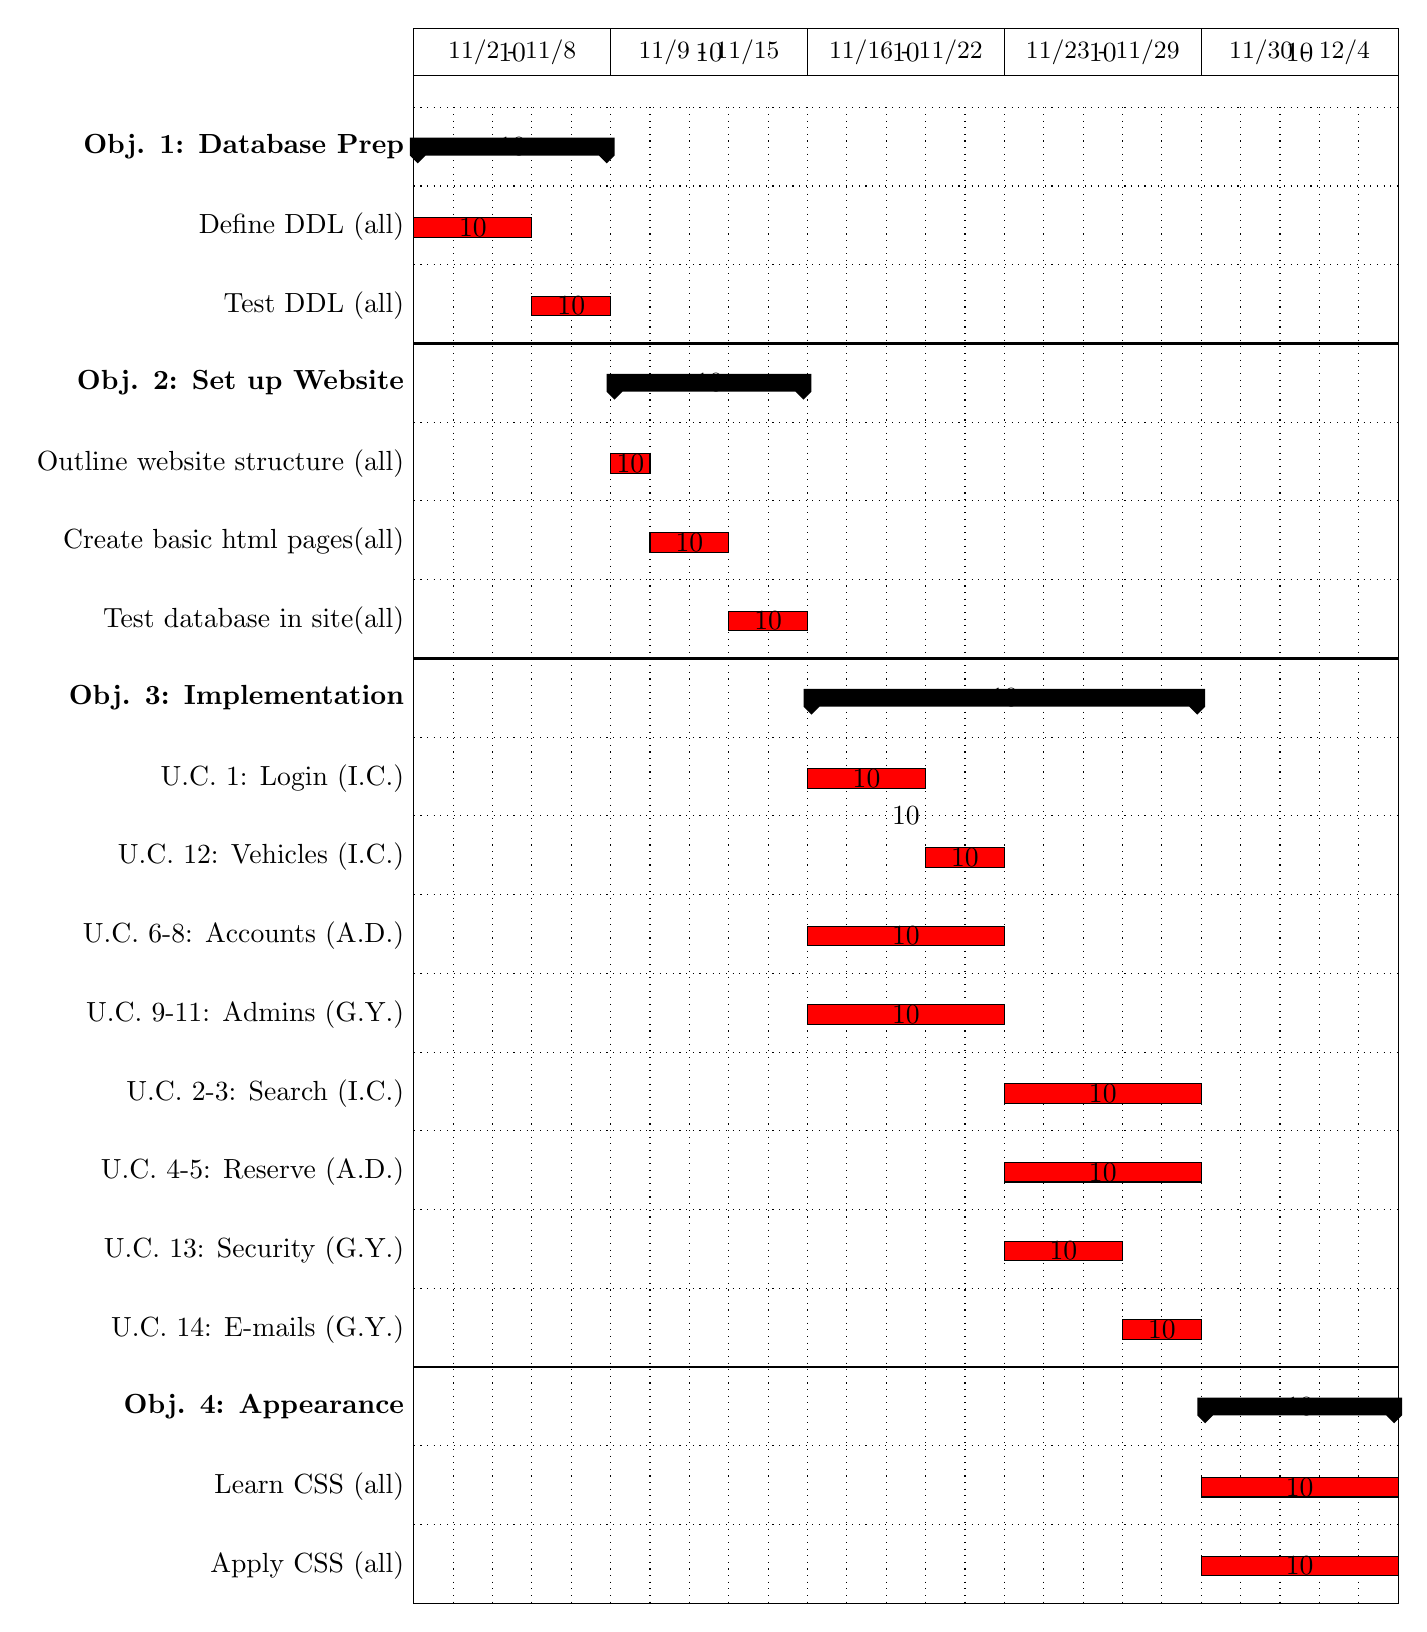
\begin{tikzpicture}
\tikzstyle{every node} = [font=10]
\begin{ganttchart}[hgrid,vgrid, bar/.append style={fill=red}, bar height = .25, bar top shift = .4]{1}{25} 
	\gantttitle{11/2 - 11/8}{5}  %title, length of title
	\gantttitle{11/9 - 11/15}{5}
	\gantttitle{11/16 - 11/22}{5} 
	\gantttitle{11/23 - 11/29}{5}
	\gantttitle{11/30 - 12/4}{5} \\

	\ganttgroup{Obj. 1: Database Prep}{1}{5} \\ %title, start, end
	\ganttbar{Define DDL (all)}{1}{3} \\
	\ganttbar{Test DDL (all)}{4}{5} \ganttnewline[thick]

	\ganttgroup{Obj. 2: Set up Website}{6}{10} \\
	\ganttbar{Outline website structure (all)}{6}{6} \\
	\ganttbar{Create basic html pages(all)}{7}{8} \\
	\ganttbar{Test database in site(all)}{9}{10} \ganttnewline[thick]

	\ganttgroup{Obj. 3: Implementation}{11}{20} \\
	\ganttbar{U.C. 1: Login (I.C.)}{11}{13} \\
	\ganttbar{U.C. 12: Vehicles (I.C.)}{14}{15} \\
	\ganttbar{U.C. 6-8: Accounts (A.D.)}{11}{15} \\
	\ganttbar{U.C. 9-11: Admins (G.Y.)}{11}{15} \\
	\ganttbar{U.C. 2-3: Search (I.C.)}{16}{20} \\
	\ganttbar{U.C. 4-5: Reserve (A.D.)}{16}{20} \\
	\ganttbar{U.C. 13: Security (G.Y.)}{16}{18} \\
	\ganttbar{U.C. 14: E-mails (G.Y.)}{19}{20} \ganttnewline[thick]

	\ganttgroup{Obj. 4: Appearance}{21}{25} \\
	\ganttbar{Learn CSS (all)}{21}{25} \\
	\ganttbar{Apply CSS (all)}{21}{25}
\end{ganttchart}
\end{tikzpicture}
}

\section{ER Diagram}

\includegraphics[scale=0.8]{CarRentalERDiagram.pdf}

\section{Schema Diagram}

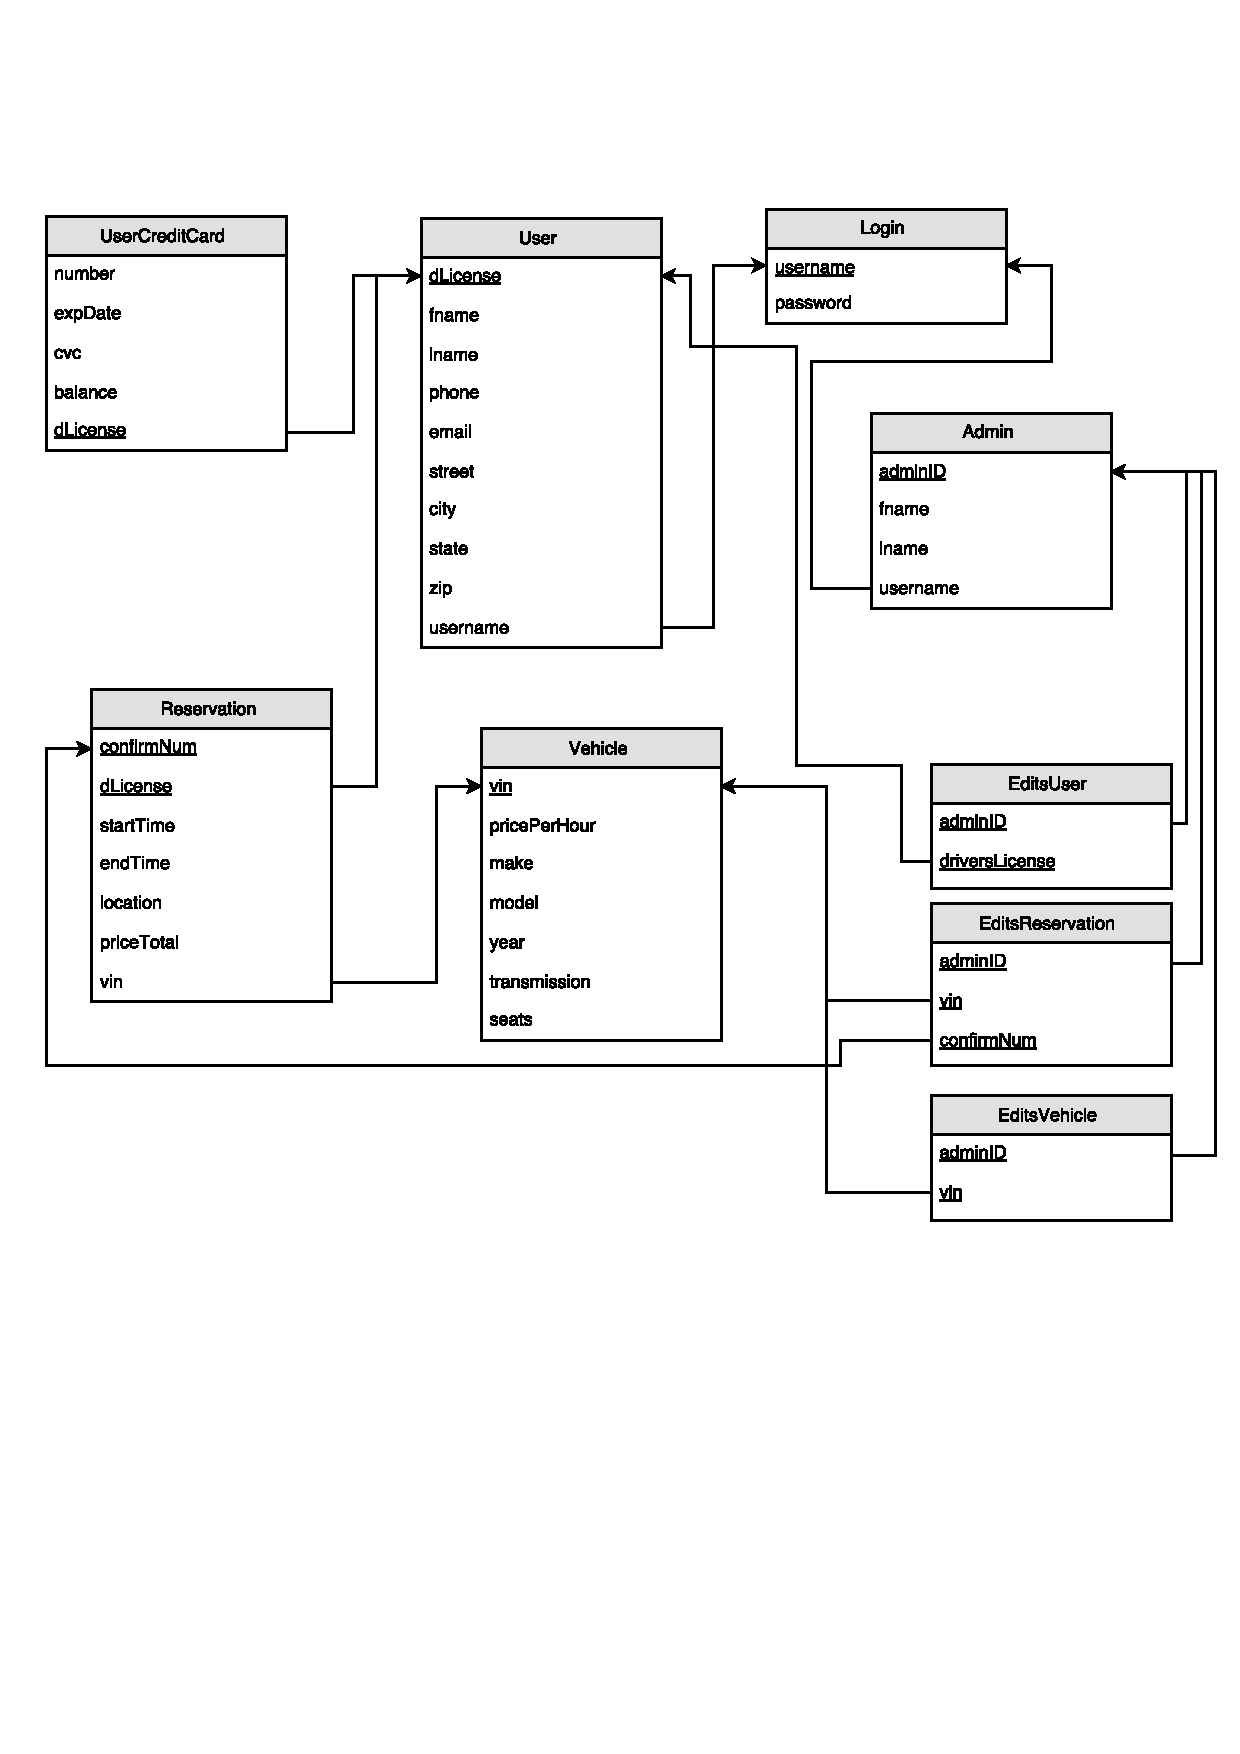
\includegraphics[scale=0.8]{carRentalSchema.pdf}

\end{document}